\documentclass[../main.tex]{subfiles}
\captionsetup[subfloat]{labelformat=empty}
\begin{document}

\chapter{First validation test for QCD estimation}
\label{appendix_b}

\renewcommand{\thefigure}{B.\arabic{figure}}

This appendix shows the results for the C/D yield estimation, corresponding to the first QCD validation test, in all years (2016, 2017, and 2018) and $\tau\tau$ decay channels. This test is fully described in Section~\ref{hh:sec:validation_qcd}.


\begin{figure}[h!]
    \begin{center}

    \subfloat[Boosted]{\includegraphics[width=0.4\textwidth]{Images/qcd_tests/2016/boosted/qcd_inviso__mutau.pdf}}
    \subfloat[Resolved 1 b-tag]{\includegraphics[width=0.4\textwidth]{Images/qcd_tests/2016/resolved_1b/qcd_inviso__mutau.pdf}}\\
    \subfloat[Resolved 2 b-tag]{\includegraphics[width=0.4\textwidth]{Images/qcd_tests/2016/resolved_2b/qcd_inviso__mutau.pdf}}
    \subfloat[VBF subcategory]{\includegraphics[width=0.4\textwidth]{Images/qcd_tests/2016/vbf/hh_vbf_sm_c2v/qcd_inviso__mutau.pdf}}\\
    \subfloat[ggF subcategory]{\includegraphics[width=0.4\textwidth]{Images/qcd_tests/2016/vbf/hh_ggf/qcd_inviso__mutau.pdf}}
    \subfloat[\ttbar{} subcategory]{\includegraphics[width=0.4\textwidth]{Images/qcd_tests/2016/vbf/tt/qcd_inviso__mutau.pdf}}\\
    \subfloat[\tth{} subcategory]{\includegraphics[width=0.4\textwidth]{Images/qcd_tests/2016/vbf/ttH/qcd_inviso__mutau.pdf}}
    \subfloat[DY subcategory]{\includegraphics[width=0.4\textwidth]{Images/qcd_tests/2016/vbf/dy/qcd_inviso__mutau.pdf}}

    \caption[First validity test results for the QCD estimation for the \taumu\tauh{} channel in 2016]{C/D yield estimations for the five working points for the \taumu\tauh{} channel in 2016. A dashed band is plotted where the correspondent working point leads to a negative yield for regions B, C and/or D.}

    \end{center}
\end{figure}


\begin{figure}[h!]
    \begin{center}

    \subfloat[Boosted]{\includegraphics[width=0.4\textwidth]{Images/qcd_tests/2016/boosted/qcd_inviso__etau.pdf}}
    \subfloat[Resolved 1 b-tag]{\includegraphics[width=0.4\textwidth]{Images/qcd_tests/2016/resolved_1b/qcd_inviso__etau.pdf}}\\
    \subfloat[Resolved 2 b-tag]{\includegraphics[width=0.4\textwidth]{Images/qcd_tests/2016/resolved_2b/qcd_inviso__etau.pdf}}
    \subfloat[VBF subcategory]{\includegraphics[width=0.4\textwidth]{Images/qcd_tests/2016/vbf/hh_vbf_sm_c2v/qcd_inviso__etau.pdf}}\\
    \subfloat[ggF subcategory]{\includegraphics[width=0.4\textwidth]{Images/qcd_tests/2016/vbf/hh_ggf/qcd_inviso__etau.pdf}}
    \subfloat[\ttbar{} subcategory]{\includegraphics[width=0.4\textwidth]{Images/qcd_tests/2016/vbf/tt/qcd_inviso__etau.pdf}}\\
    \subfloat[\tth{} subcategory]{\includegraphics[width=0.4\textwidth]{Images/qcd_tests/2016/vbf/ttH/qcd_inviso__etau.pdf}}
    \subfloat[DY subcategory]{\includegraphics[width=0.4\textwidth]{Images/qcd_tests/2016/vbf/dy/qcd_inviso__etau.pdf}}

    \caption[First validity test results for the QCD estimation for the \taue\tauh{} channel in 2016]{C/D yield estimations for the five working points for the \taue\tauh{} channel in 2016. A dashed band is plotted where the correspondent working point leads to a negative yield for regions B, C and/or D.}

    \end{center}
\end{figure}


\begin{figure}[h!]
    \begin{center}

    \subfloat[Boosted]{\includegraphics[width=0.4\textwidth]{Images/qcd_tests/2016/boosted/qcd_inviso__tautau.pdf}}
    \subfloat[Resolved 1 b-tag]{\includegraphics[width=0.4\textwidth]{Images/qcd_tests/2016/resolved_1b/qcd_inviso__tautau.pdf}}\\
    \subfloat[Resolved 2 b-tag]{\includegraphics[width=0.4\textwidth]{Images/qcd_tests/2016/resolved_2b/qcd_inviso__tautau.pdf}}
    \subfloat[VBF subcategory]{\includegraphics[width=0.4\textwidth]{Images/qcd_tests/2016/vbf/hh_vbf_sm_c2v/qcd_inviso__tautau.pdf}}\\
    \subfloat[ggF subcategory]{\includegraphics[width=0.4\textwidth]{Images/qcd_tests/2016/vbf/hh_ggf/qcd_inviso__tautau.pdf}}
    \subfloat[\ttbar{} subcategory]{\includegraphics[width=0.4\textwidth]{Images/qcd_tests/2016/vbf/tt/qcd_inviso__tautau.pdf}}\\
    \subfloat[\tth{} subcategory]{\includegraphics[width=0.4\textwidth]{Images/qcd_tests/2016/vbf/ttH/qcd_inviso__tautau.pdf}}
    \subfloat[DY subcategory]{\includegraphics[width=0.4\textwidth]{Images/qcd_tests/2016/vbf/dy/qcd_inviso__tautau.pdf}}

    \caption[First validity test results for the QCD estimation for the \tauh\tauh{} channel in 2016]{C/D yield estimations for the five working points for the \tauh\tauh{} channel in 2016. A dashed band is plotted where the correspondent working point leads to a negative yield for regions B, C and/or D.}

    \end{center}
\end{figure}


\begin{figure}[h!]
    \begin{center}

    \subfloat[Boosted]{\includegraphics[width=0.4\textwidth]{Images/qcd_tests/2017/boosted/qcd_inviso__mutau.pdf}}
    \subfloat[Resolved 1 b-tag]{\includegraphics[width=0.4\textwidth]{Images/qcd_tests/2017/resolved_1b/qcd_inviso__mutau.pdf}}\\
    \subfloat[Resolved 2 b-tag]{\includegraphics[width=0.4\textwidth]{Images/qcd_tests/2017/resolved_2b/qcd_inviso__mutau.pdf}}
    \subfloat[VBF subcategory]{\includegraphics[width=0.4\textwidth]{Images/qcd_tests/2017/vbf/hh_vbf_sm_c2v/qcd_inviso__mutau.pdf}}\\
    \subfloat[ggF subcategory]{\includegraphics[width=0.4\textwidth]{Images/qcd_tests/2017/vbf/hh_ggf/qcd_inviso__mutau.pdf}}
    \subfloat[\ttbar{} subcategory]{\includegraphics[width=0.4\textwidth]{Images/qcd_tests/2017/vbf/tt/qcd_inviso__mutau.pdf}}\\
    \subfloat[\tth{} subcategory]{\includegraphics[width=0.4\textwidth]{Images/qcd_tests/2017/vbf/ttH/qcd_inviso__mutau.pdf}}
    \subfloat[DY subcategory]{\includegraphics[width=0.4\textwidth]{Images/qcd_tests/2017/vbf/dy/qcd_inviso__mutau.pdf}}

    \caption[First validity test results for the QCD estimation for the \taumu\tauh{} channel in 2017]{C/D yield estimations for the five working points for the \taumu\tauh{} channel in 2017. A dashed band is plotted where the correspondent working point leads to a negative yield for regions B, C and/or D.}

    \end{center}
\end{figure}


\begin{figure}[h!]
    \begin{center}

    \subfloat[Boosted]{\includegraphics[width=0.4\textwidth]{Images/qcd_tests/2017/boosted/qcd_inviso__etau.pdf}}
    \subfloat[Resolved 1 b-tag]{\includegraphics[width=0.4\textwidth]{Images/qcd_tests/2017/resolved_1b/qcd_inviso__etau.pdf}}\\
    \subfloat[Resolved 2 b-tag]{\includegraphics[width=0.4\textwidth]{Images/qcd_tests/2017/resolved_2b/qcd_inviso__etau.pdf}}
    \subfloat[VBF subcategory]{\includegraphics[width=0.4\textwidth]{Images/qcd_tests/2017/vbf/hh_vbf_sm_c2v/qcd_inviso__etau.pdf}}\\
    \subfloat[ggF subcategory]{\includegraphics[width=0.4\textwidth]{Images/qcd_tests/2017/vbf/hh_ggf/qcd_inviso__etau.pdf}}
    \subfloat[\ttbar{} subcategory]{\includegraphics[width=0.4\textwidth]{Images/qcd_tests/2017/vbf/tt/qcd_inviso__etau.pdf}}\\
    \subfloat[\tth{} subcategory]{\includegraphics[width=0.4\textwidth]{Images/qcd_tests/2017/vbf/ttH/qcd_inviso__etau.pdf}}
    \subfloat[DY subcategory]{\includegraphics[width=0.4\textwidth]{Images/qcd_tests/2017/vbf/dy/qcd_inviso__etau.pdf}}

    \caption[First validity test results for the QCD estimation for the \taue\tauh{} channel in 2017]{C/D yield estimations for the five working points for the \taue\tauh{} channel in 2017. A dashed band is plotted where the correspondent working point leads to a negative yield for regions B, C and/or D.}

    \end{center}
\end{figure}


\begin{figure}[h!]
    \begin{center}

    \subfloat[Boosted]{\includegraphics[width=0.4\textwidth]{Images/qcd_tests/2017/boosted/qcd_inviso__tautau.pdf}}
    \subfloat[Resolved 1 b-tag]{\includegraphics[width=0.4\textwidth]{Images/qcd_tests/2017/resolved_1b/qcd_inviso__tautau.pdf}}\\
    \subfloat[Resolved 2 b-tag]{\includegraphics[width=0.4\textwidth]{Images/qcd_tests/2017/resolved_2b/qcd_inviso__tautau.pdf}}
    \subfloat[VBF subcategory]{\includegraphics[width=0.4\textwidth]{Images/qcd_tests/2017/vbf/hh_vbf_sm_c2v/qcd_inviso__tautau.pdf}}\\
    \subfloat[ggF subcategory]{\includegraphics[width=0.4\textwidth]{Images/qcd_tests/2017/vbf/hh_ggf/qcd_inviso__tautau.pdf}}
    \subfloat[\ttbar{} subcategory]{\includegraphics[width=0.4\textwidth]{Images/qcd_tests/2017/vbf/tt/qcd_inviso__tautau.pdf}}\\
    \subfloat[\tth{} subcategory]{\includegraphics[width=0.4\textwidth]{Images/qcd_tests/2017/vbf/ttH/qcd_inviso__tautau.pdf}}
    \subfloat[DY subcategory]{\includegraphics[width=0.4\textwidth]{Images/qcd_tests/2017/vbf/dy/qcd_inviso__tautau.pdf}}

    \caption[First validity test results for the QCD estimation for the \tauh\tauh{} channel in 2017]{C/D yield estimations for the five working points for the \tauh\tauh{} channel in 2017. A dashed band is plotted where the correspondent working point leads to a negative yield for regions B, C and/or D.}

    \end{center}
\end{figure}


\begin{figure}[h!]
    \begin{center}

    \subfloat[Boosted]{\includegraphics[width=0.4\textwidth]{Images/qcd_tests/2018/boosted/qcd_inviso__mutau.pdf}}
    \subfloat[Resolved 1 b-tag]{\includegraphics[width=0.4\textwidth]{Images/qcd_tests/2018/resolved_1b/qcd_inviso__mutau.pdf}}\\
    \subfloat[Resolved 2 b-tag]{\includegraphics[width=0.4\textwidth]{Images/qcd_tests/2018/resolved_2b/qcd_inviso__mutau.pdf}}
    \subfloat[VBF subcategory]{\includegraphics[width=0.4\textwidth]{Images/qcd_tests/2018/vbf/hh_vbf_sm_c2v/qcd_inviso__mutau.pdf}}\\
    \subfloat[ggF subcategory]{\includegraphics[width=0.4\textwidth]{Images/qcd_tests/2018/vbf/hh_ggf/qcd_inviso__mutau.pdf}}
    \subfloat[\ttbar{} subcategory]{\includegraphics[width=0.4\textwidth]{Images/qcd_tests/2018/vbf/tt/qcd_inviso__mutau.pdf}}\\
    \subfloat[\tth{} subcategory]{\includegraphics[width=0.4\textwidth]{Images/qcd_tests/2018/vbf/ttH/qcd_inviso__mutau.pdf}}
    \subfloat[DY subcategory]{\includegraphics[width=0.4\textwidth]{Images/qcd_tests/2018/vbf/dy/qcd_inviso__mutau.pdf}}

    \caption[First validity test results for the QCD estimation for the \taumu\tauh{} channel in 2018]{C/D yield estimations for the five working points for the \taumu\tauh{} channel in 2018. A dashed band is plotted where the correspondent working point leads to a negative yield for regions B, C and/or D.}

    \end{center}
\end{figure}


\begin{figure}[h!]
    \begin{center}

    \subfloat[Boosted]{\includegraphics[width=0.4\textwidth]{Images/qcd_tests/2018/boosted/qcd_inviso__etau.pdf}}
    \subfloat[Resolved 1 b-tag]{\includegraphics[width=0.4\textwidth]{Images/qcd_tests/2018/resolved_1b/qcd_inviso__etau.pdf}}\\
    \subfloat[Resolved 2 b-tag]{\includegraphics[width=0.4\textwidth]{Images/qcd_tests/2018/resolved_2b/qcd_inviso__etau.pdf}}
    \subfloat[VBF subcategory]{\includegraphics[width=0.4\textwidth]{Images/qcd_tests/2018/vbf/hh_vbf_sm_c2v/qcd_inviso__etau.pdf}}\\
    \subfloat[ggF subcategory]{\includegraphics[width=0.4\textwidth]{Images/qcd_tests/2018/vbf/hh_ggf/qcd_inviso__etau.pdf}}
    \subfloat[\ttbar{} subcategory]{\includegraphics[width=0.4\textwidth]{Images/qcd_tests/2018/vbf/tt/qcd_inviso__etau.pdf}}\\
    \subfloat[\tth{} subcategory]{\includegraphics[width=0.4\textwidth]{Images/qcd_tests/2018/vbf/ttH/qcd_inviso__etau.pdf}}
    \subfloat[DY subcategory]{\includegraphics[width=0.4\textwidth]{Images/qcd_tests/2018/vbf/dy/qcd_inviso__etau.pdf}}

    \caption[First validity test results for the QCD estimation for the \taue\tauh{} channel in 2018]{C/D yield estimations for the five working points for the \taue\tauh{} channel in 2018. A dashed band is plotted where the correspondent working point leads to a negative yield for regions B, C and/or D.}

    \end{center}
\end{figure}


\begin{figure}[h!]
    \begin{center}

    \subfloat[Boosted]{\includegraphics[width=0.4\textwidth]{Images/qcd_tests/2018/boosted/qcd_inviso__tautau.pdf}}
    \subfloat[Resolved 1 b-tag]{\includegraphics[width=0.4\textwidth]{Images/qcd_tests/2018/resolved_1b/qcd_inviso__tautau.pdf}}\\
    \subfloat[Resolved 2 b-tag]{\includegraphics[width=0.4\textwidth]{Images/qcd_tests/2018/resolved_2b/qcd_inviso__tautau.pdf}}
    \subfloat[VBF subcategory]{\includegraphics[width=0.4\textwidth]{Images/qcd_tests/2018/vbf/hh_vbf_sm_c2v/qcd_inviso__tautau.pdf}}\\
    \subfloat[ggF subcategory]{\includegraphics[width=0.4\textwidth]{Images/qcd_tests/2018/vbf/hh_ggf/qcd_inviso__tautau.pdf}}
    \subfloat[\ttbar{} subcategory]{\includegraphics[width=0.4\textwidth]{Images/qcd_tests/2018/vbf/tt/qcd_inviso__tautau.pdf}}\\
    \subfloat[\tth{} subcategory]{\includegraphics[width=0.4\textwidth]{Images/qcd_tests/2018/vbf/ttH/qcd_inviso__tautau.pdf}}
    \subfloat[DY subcategory]{\includegraphics[width=0.4\textwidth]{Images/qcd_tests/2018/vbf/dy/qcd_inviso__tautau.pdf}}

    \caption[First validity test results for the QCD estimation for the \tauh\tauh{} channel in 2018]{C/D yield estimations for the five working points for the \tauh\tauh{} channel in 2018. A dashed band is plotted where the correspondent working point leads to a negative yield for regions B, C and/or D.}

    \end{center}
\end{figure}










\end{document}

